%!TEX program = pdflatex
\documentclass[11pt,en]{elegantpaper}

\title{Report for the Project}
\author{Wenchong Huang}

\date{\today}

% cmd for this doc
\usepackage{array}
\usepackage{float}
\usepackage{pgfplots}
\usepackage{tikz}
\usepackage{graphicx}
\usepackage{subfigure}
\newcommand{\ccr}[1]{\makecell{{\color{#1}\rule{1cm}{1cm}}}}

\begin{document}

\maketitle

\section{Introduction}

This project is a simple implemention of piecewise spline interpolation, including linear and cubic. Both are implemented with two different algorithm: ppForm and B-SPline.

For the cubic spline interpolation, five different bondary conditions are supported.

\begin{itemize}
    \item \textit{natural}: $s''(t_1)=s''(t_N)=0$.
    \item \textit{complete}: $s'(t_1)=f'(t_1),\;s'(t_N)=f'(t_N)$.
    \item \textit{second-derivatives-at-end}: $s''(t_1)=f''(t_1),\;s''(t_N)=f''(t_N)$.
    \item \textit{periodic}: $s'(t_1)=s'(t_N),\;s''(t_1)=s''(t_N)$.
    \item \textit{not-a-knot}: $s'''(t_2)$ and $s'''(t_{N-1})$ exist.
\end{itemize}

\textit{natural}, \textit{complete}, \textit{second-derivatives-at-end} and \textit{periodic} are supported in both ppForm and B-Spline. And \textit{not-a-knot} is only supported in ppForm.

For how to use the interpolators, see the document. For how to test, firstly \textbf{run} \verb|make| \textbf{in the sorce code directory}, then read this report to see how to test.

\section{Function Test}

\subsection{Function Fitting}

In this part, we use Runge's function as the example. The results see figure 1-4. Run

\begin{lstlisting}
    ./runge_ppForm > ppForm.txt
    ./runge_BSpline > BSpline.txt
\end{lstlisting}

to get the numerical results in two text files. Copy all the text in \verb|ppForm.txt|, replace line 3-7 of \verb|draw_ppForm_cubic_function.m|. Then run the latter code with \textbf{matlab}. You will get figure 1.

To get figure 2, replace line 21-22 of \verb|test_ppForm_cubic_function.cpp| with

\begin{lstlisting}
    const int n = 11;
    const double xvalue[] = {-5, -4, -3, -2, -1, 0, 1, 2, 3, 4, 5};
\end{lstlisting}

Then run \verb|make| again, and run \verb|./runge_ppForm > ppForm.txt| again. Do the same work with \textbf{matlab}, you will see figure 2.

To get figure 3 and figure 4, do the similar work to \verb|test_BSpline_cubic_function.cpp| and \verb|draw_| \verb|BSpline_cubic_function.cpp|.

\begin{figure}[htbp]
    \begin{minipage}[t]{0.5\linewidth}
        \centering
        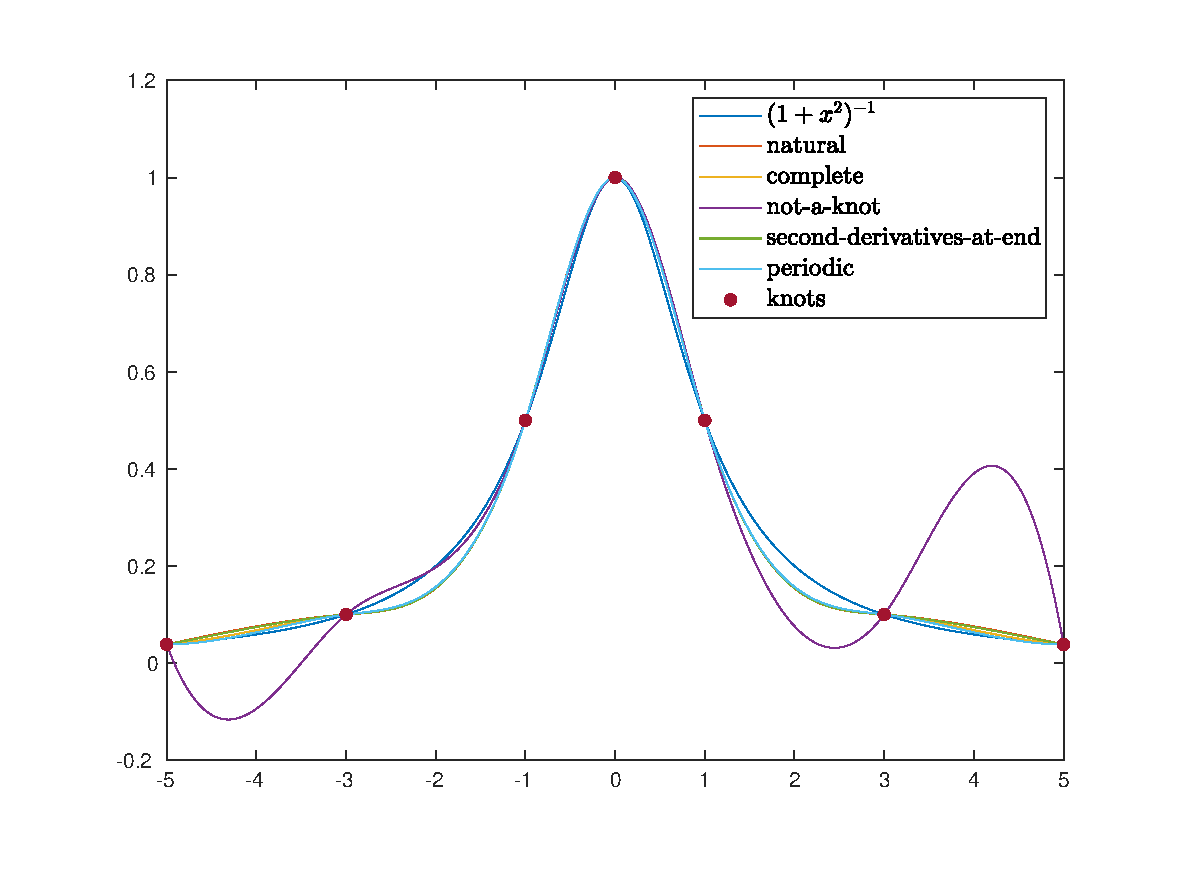
\includegraphics[width=0.9\linewidth]{figure/ppForm_7knots.eps}
        \caption{ppForm, 7 knots.}
        \label{fig:side:a}
    \end{minipage}%
    \begin{minipage}[t]{0.5\linewidth}
        \centering
        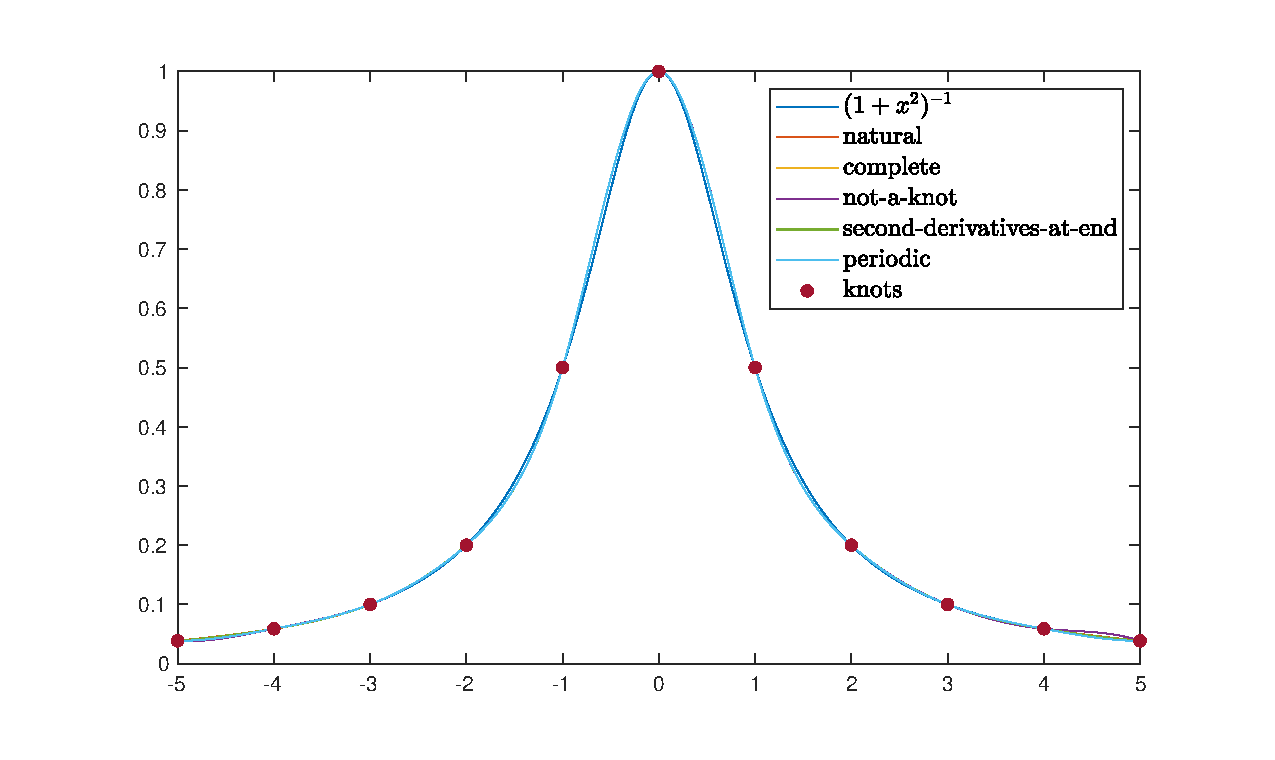
\includegraphics[width=0.9\linewidth]{figure/ppForm_11knots.eps}
        \caption{ppForm, 11 knots.}
        \label{fig:side:b}
    \end{minipage}

    \begin{minipage}[t]{0.5\linewidth}
        \centering
        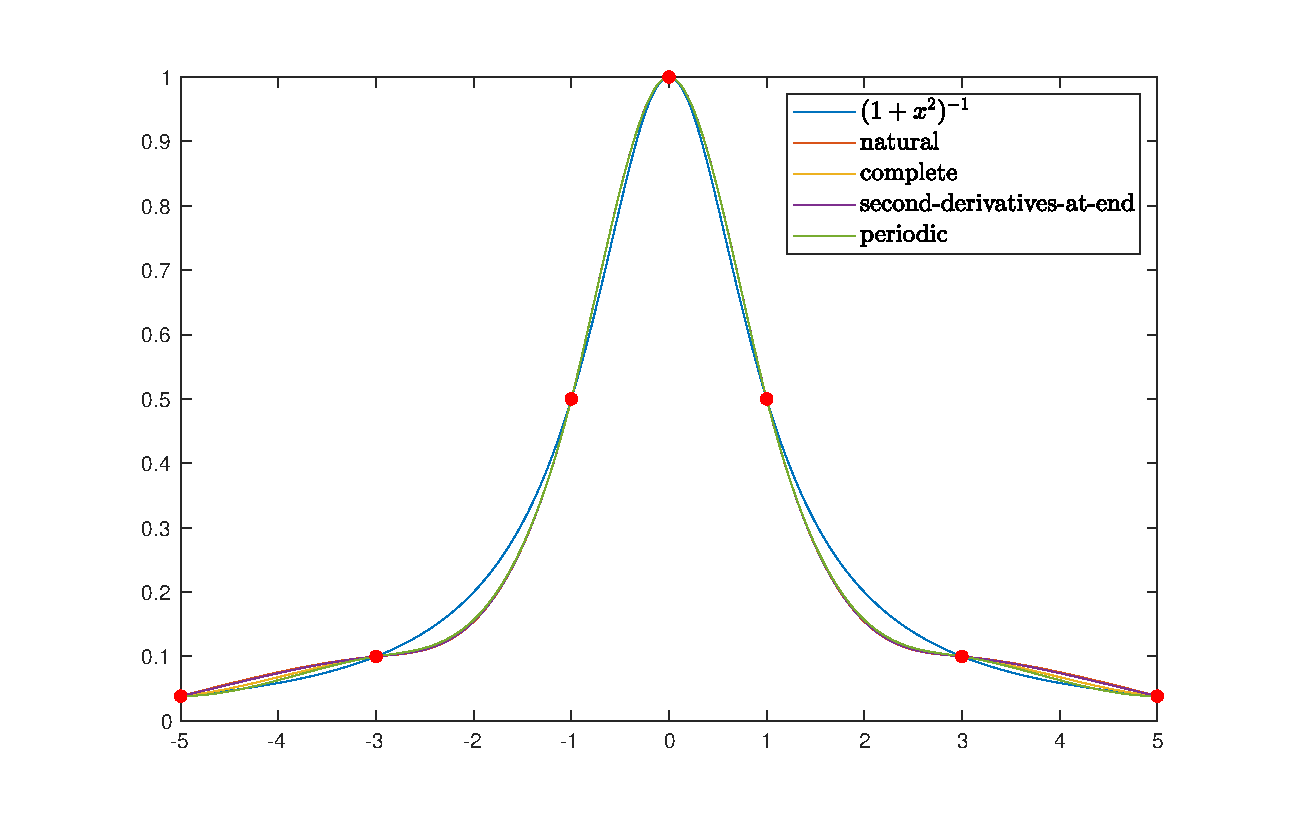
\includegraphics[width=0.9\linewidth]{figure/BSpline_7knots.eps}
        \caption{BSpline, 7 knots.}
        \label{fig:side:c}
    \end{minipage}%
    \begin{minipage}[t]{0.5\linewidth}
        \centering
        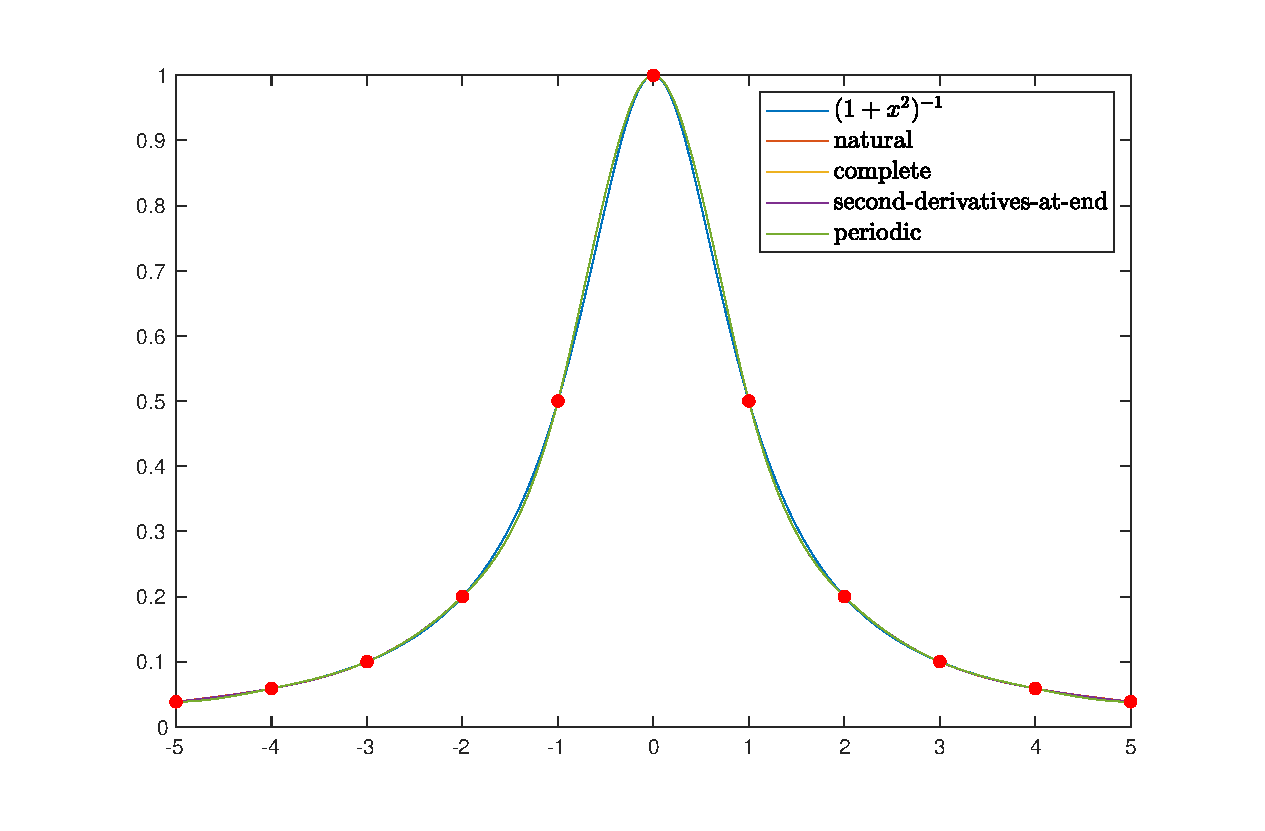
\includegraphics[width=0.9\linewidth]{figure/BSpline_11knots.eps}
        \caption{BSpline, 11 knots.}
        \label{fig:side:d}
    \end{minipage}
\end{figure}

Actually, for the same bondary condition, the interpolation results of ppForm and BSpline are the same. There's no significant difference of bondaries \textit{natural}, \textit{complete}, \textit{second-derivatives-at-end} and \textit{periodic}. But the bondary \textit{not-a-knot} performs poor when we only use 7 knots. 

\subsection{Curve Generating}

In this part, we connect some discrete points in 2D plane with a cubic spline curve. Run

\begin{lstlisting}
    ./curve > curve.txt
\end{lstlisting}

to get the numerical in a text file. Copy the text in \verb|curve.txt| and replace line 1-9 of \verb|draw_random_curve.m| with it. Run the latter code with \textbf{matlab} then you will see the result.

The result sees figure 5.

\begin{figure}[htbp]
    \centering
    \begin{minipage}[t]{0.5\linewidth}
        \centering
        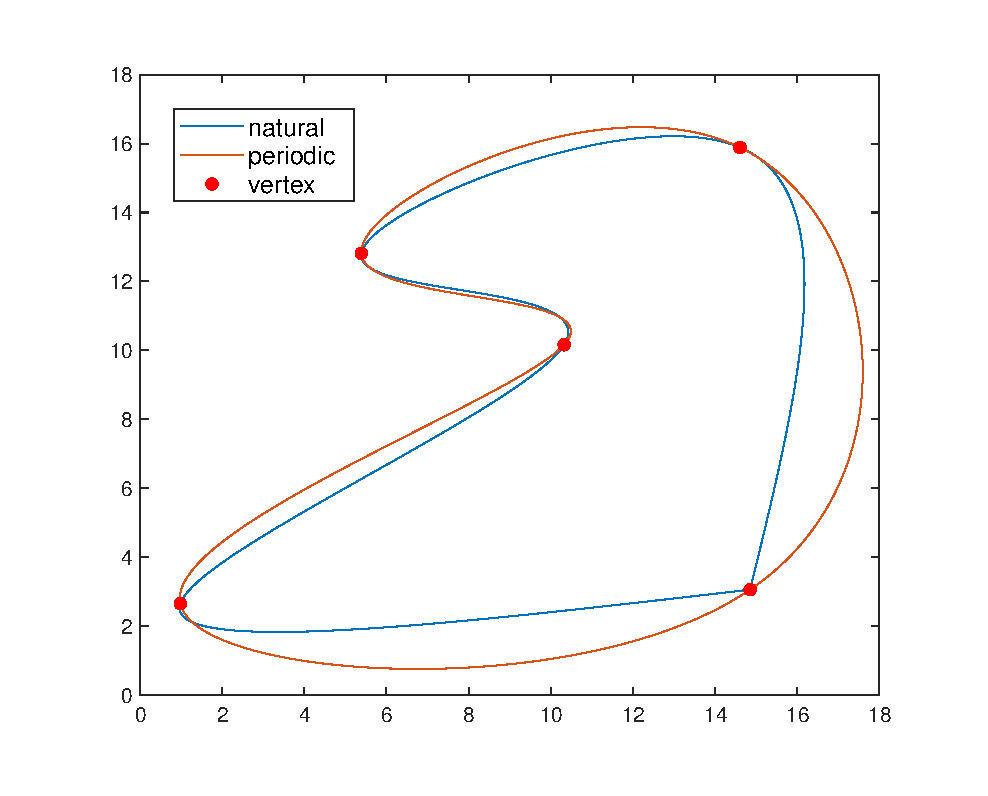
\includegraphics[width=0.7\linewidth]{figure/curve_random.eps}
        \caption{Generated cueve with discrete points.}
        \label{fig:side:a}
    \end{minipage}
\end{figure}

Two bondaries are supported. To generate closed curve, we suggest using bondary \textit{periodic}. It gives a more smooth curve than bondary \textit{natural}.

\subsection{Open Curve Fitting}

In this part, we use Helix curve $\rho=\theta$ as the example. Run

\begin{lstlisting}
    ./helix natural > natural.txt
    ./helix complete > complete.txt
    ./helix second-derivatives-at-end > sdae.txt
\end{lstlisting}

to get the numerical in text files. Copy the text and replace line 4-7 of \verb|draw_curve_helix.m| with it. Run the latter code with \textbf{matlab} then you will see the result. Use the different text to get the figure of different bondaries.

The results see figure 6-8.

\begin{figure}[htbp]
    \centering
    \begin{minipage}[t]{0.32\linewidth}
        \centering
        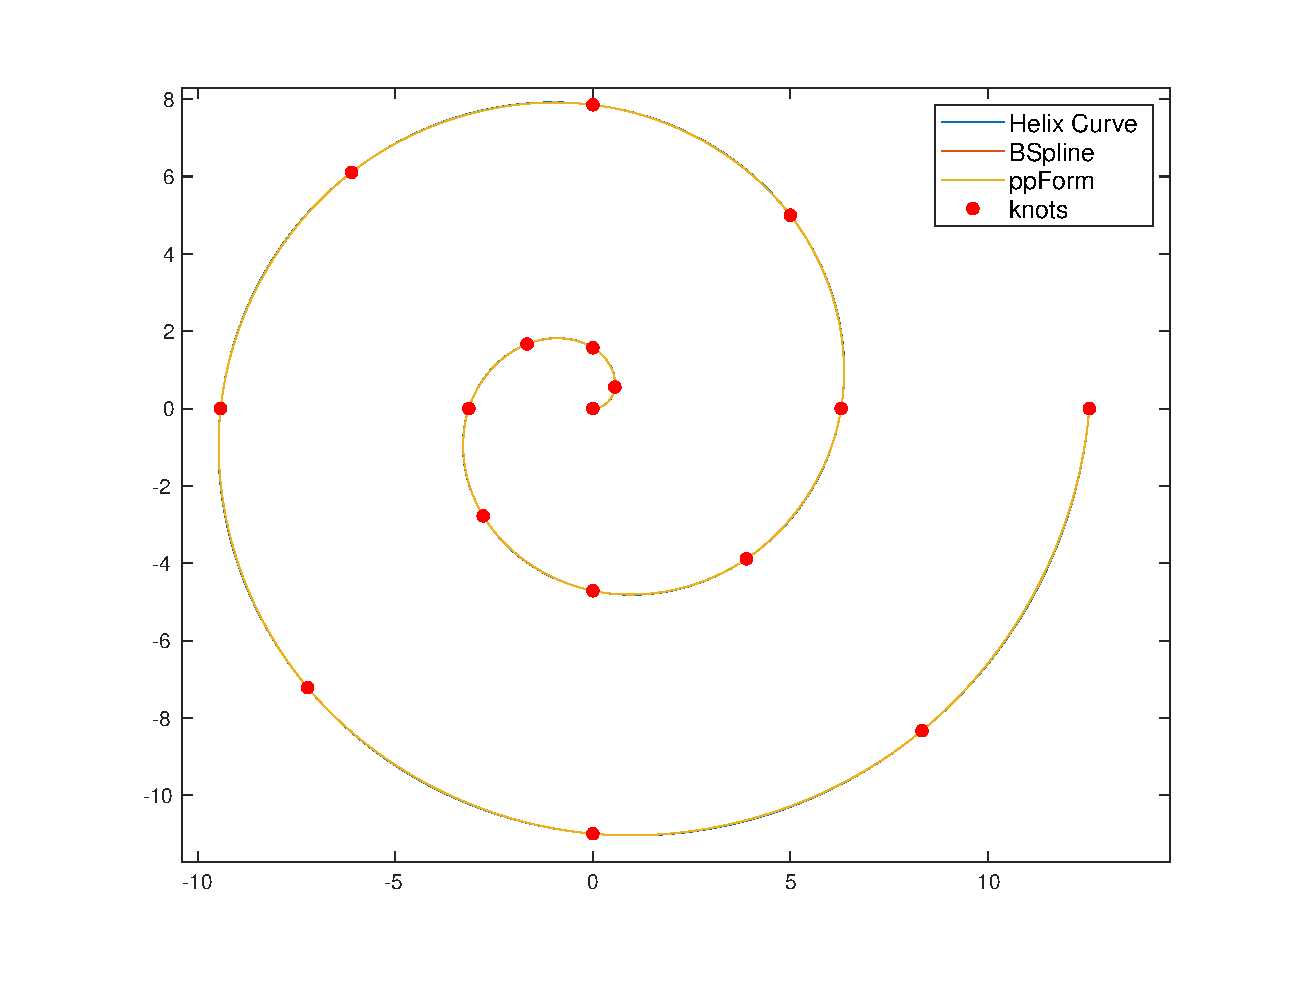
\includegraphics[width=0.9\linewidth]{figure/curve_helix_complete.eps}
        \caption{\textit{complete}}
        \label{fig:side:a}
    \end{minipage}%
    \begin{minipage}[t]{0.32\linewidth}
        \centering
        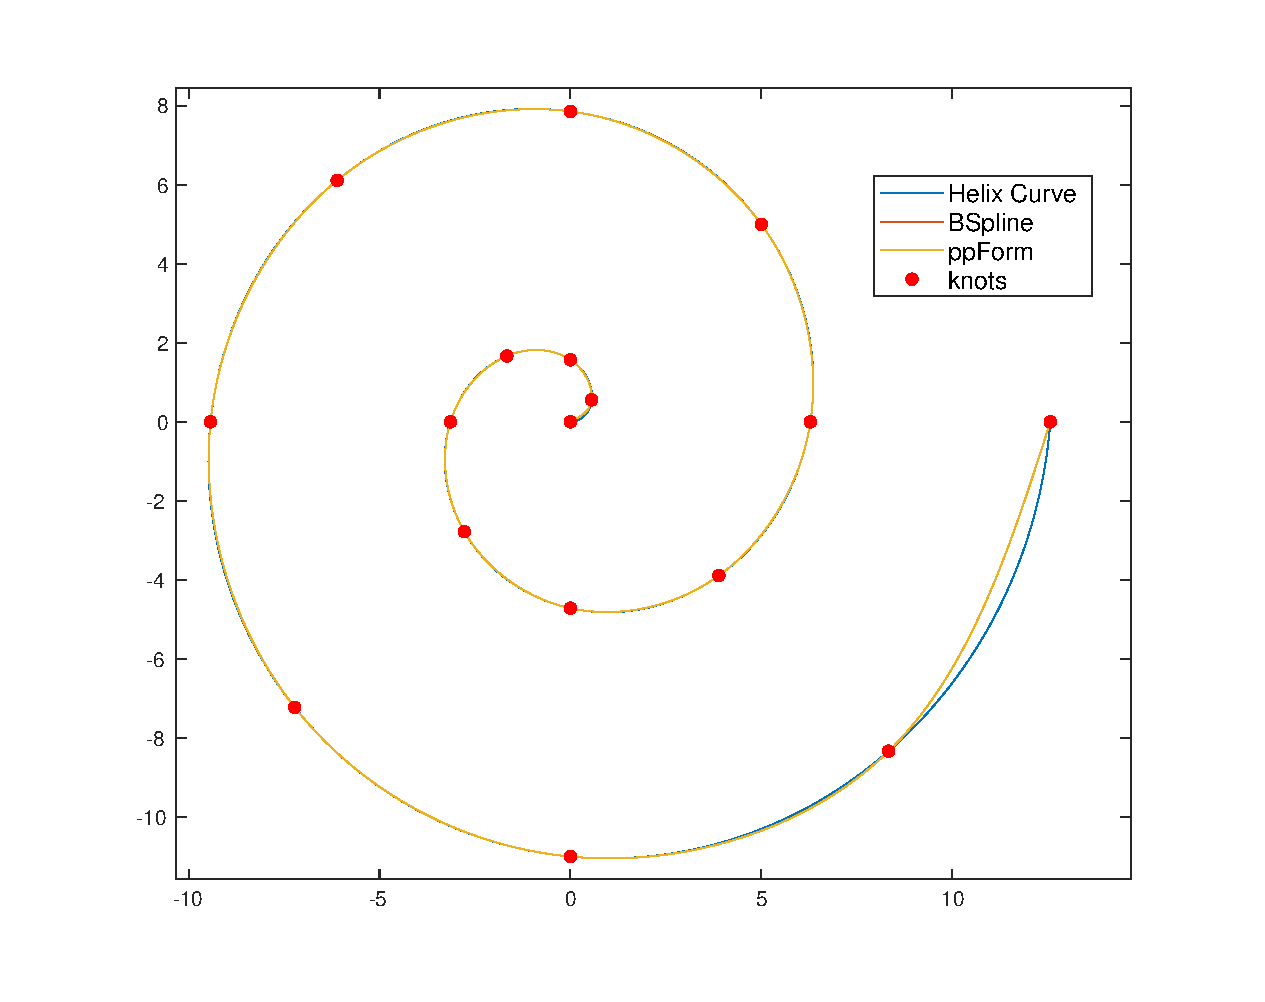
\includegraphics[width=0.9\linewidth]{figure/curve_helix_natural.eps}
        \caption{\textit{natural}}
        \label{fig:side:b}
    \end{minipage}
    \begin{minipage}[t]{0.35\linewidth}
        \centering
        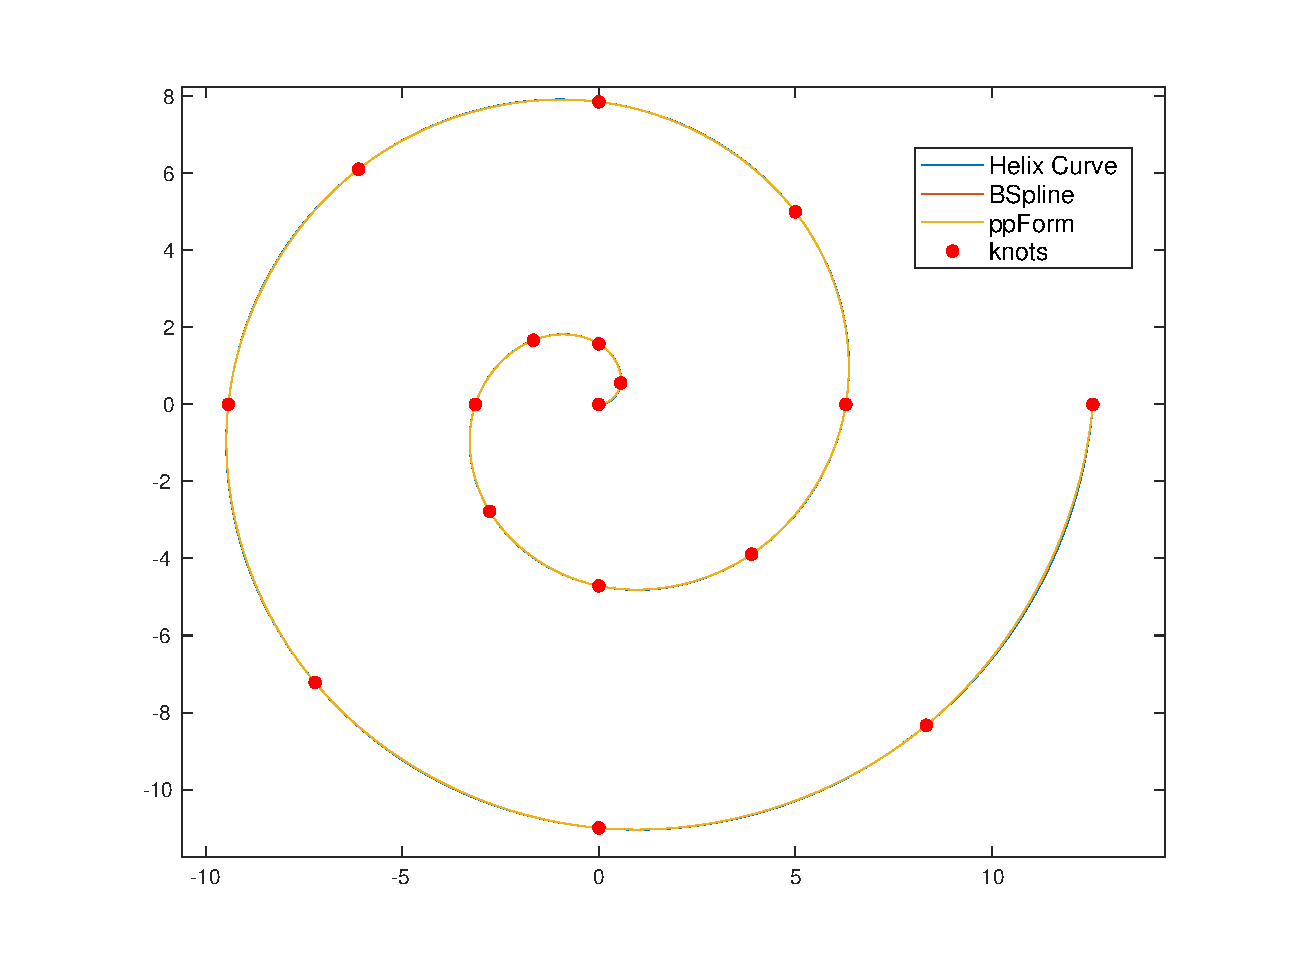
\includegraphics[width=0.9\linewidth]{figure/curve_helix_second-derivatives-at-end.eps}
        \caption{\textit{second-derivatives-at-end}}
        \label{fig:side:c}
    \end{minipage}%
\end{figure}

The bondaries \textit{complete} and \textit{second-derivatives-at-end} performs better.

\subsection{Closed Curve Fitting}

In this part we use Cardioid curve as the example. Run

\begin{lstlisting}
    ./cardioid natural > natural.txt
    ./cardioid complete > complete.txt
    ./cardioid second-derivatives-at-end > sdae.txt
    ./cardioid periodic > periodic.txt
\end{lstlisting}

to get the numerical in text files. Copy the text and replace line 4-7 of \verb|draw_curve_cardioid.m| with it. Run the latter code with \textbf{matlab} then you will see the result. Use the different text to get the figure of different bondaries.

The results see figure 9-12.

\begin{figure}[htbp]
    \centering
    \begin{minipage}[t]{0.4\linewidth}
        \centering
        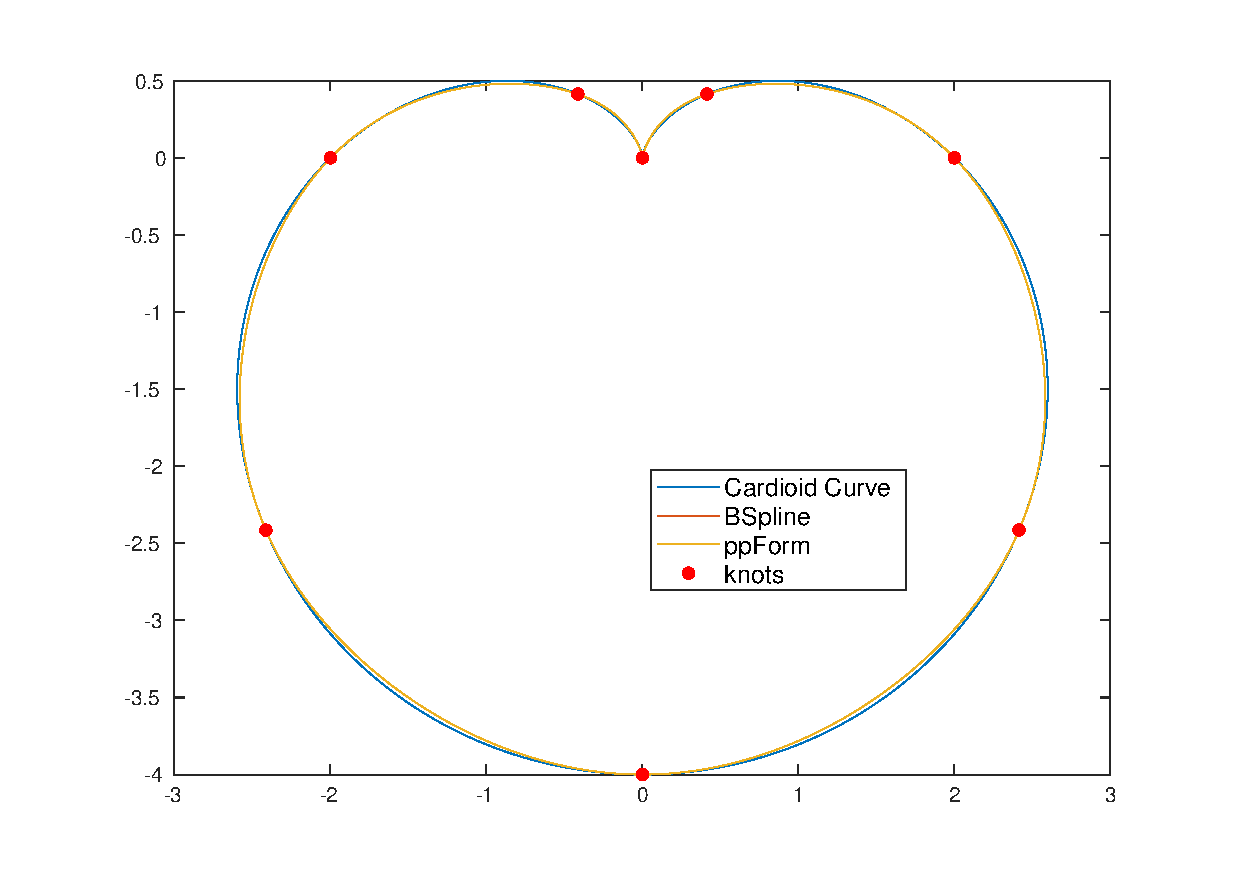
\includegraphics[width=0.9\linewidth]{figure/curve_cardioid_complete.eps}
        \caption{\textit{complete}}
        \label{fig:side:a}
    \end{minipage}%
    \begin{minipage}[t]{0.4\linewidth}
        \centering
        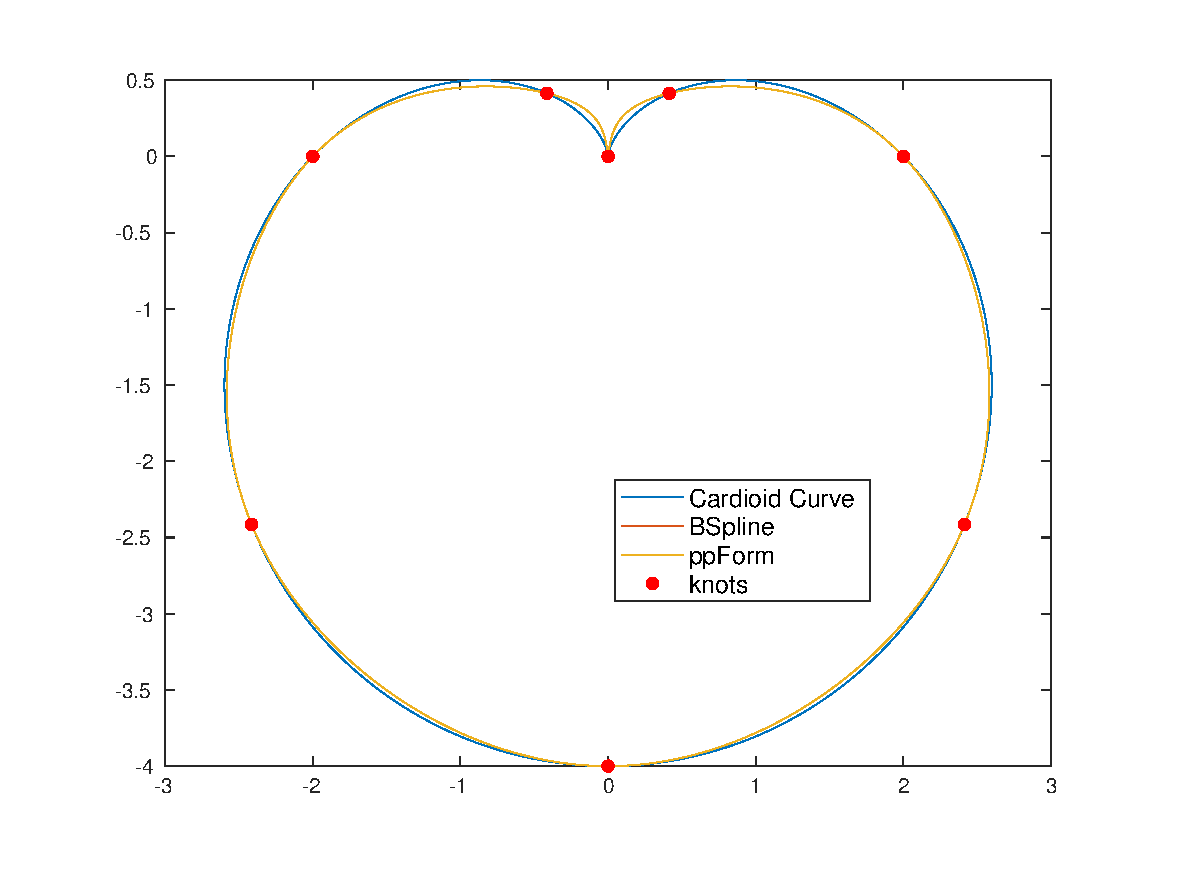
\includegraphics[width=0.9\linewidth]{figure/curve_cardioid_natural.eps}
        \caption{\textit{natural}}
        \label{fig:side:b}
    \end{minipage}
    \begin{minipage}[t]{0.4\linewidth}
        \centering
        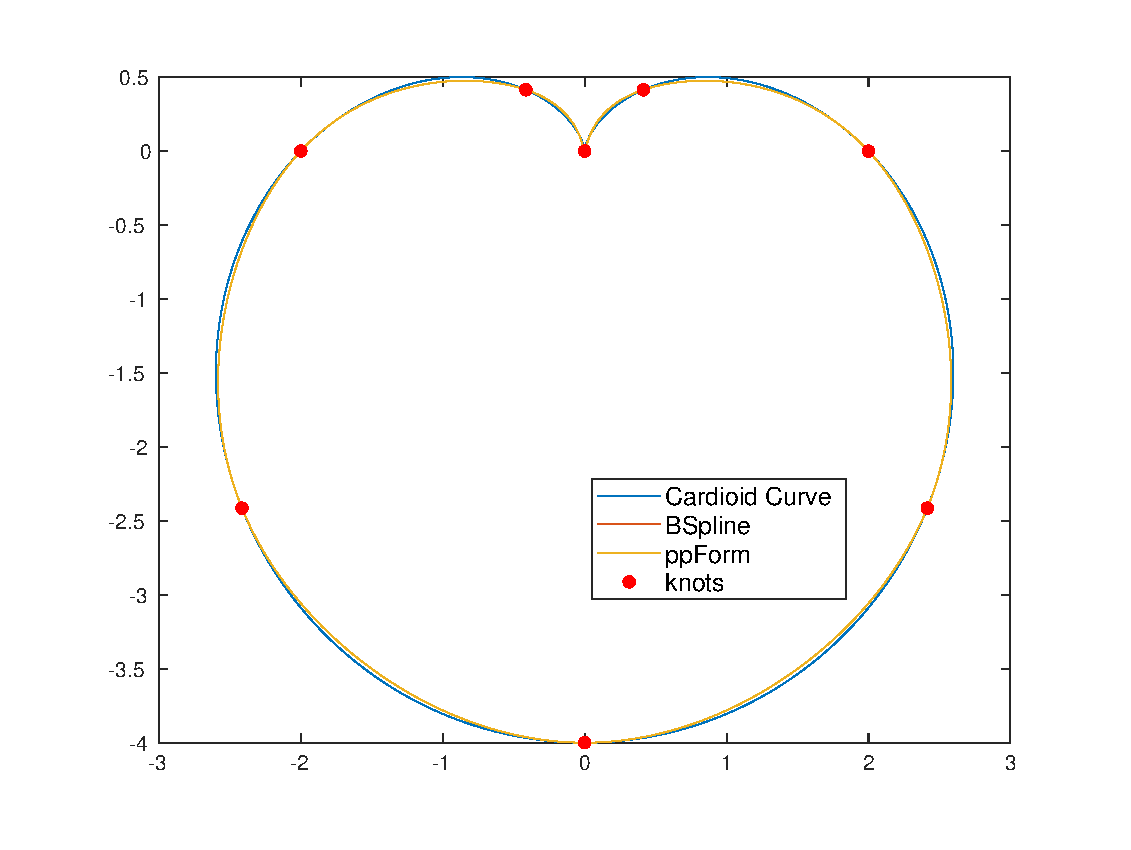
\includegraphics[width=0.9\linewidth]{figure/curve_cardioid_second-derivatives-at-end.eps}
        \caption{\textit{second-derivatives-at-end}}
        \label{fig:side:c}
    \end{minipage}%
    \begin{minipage}[t]{0.4\linewidth}
        \centering
        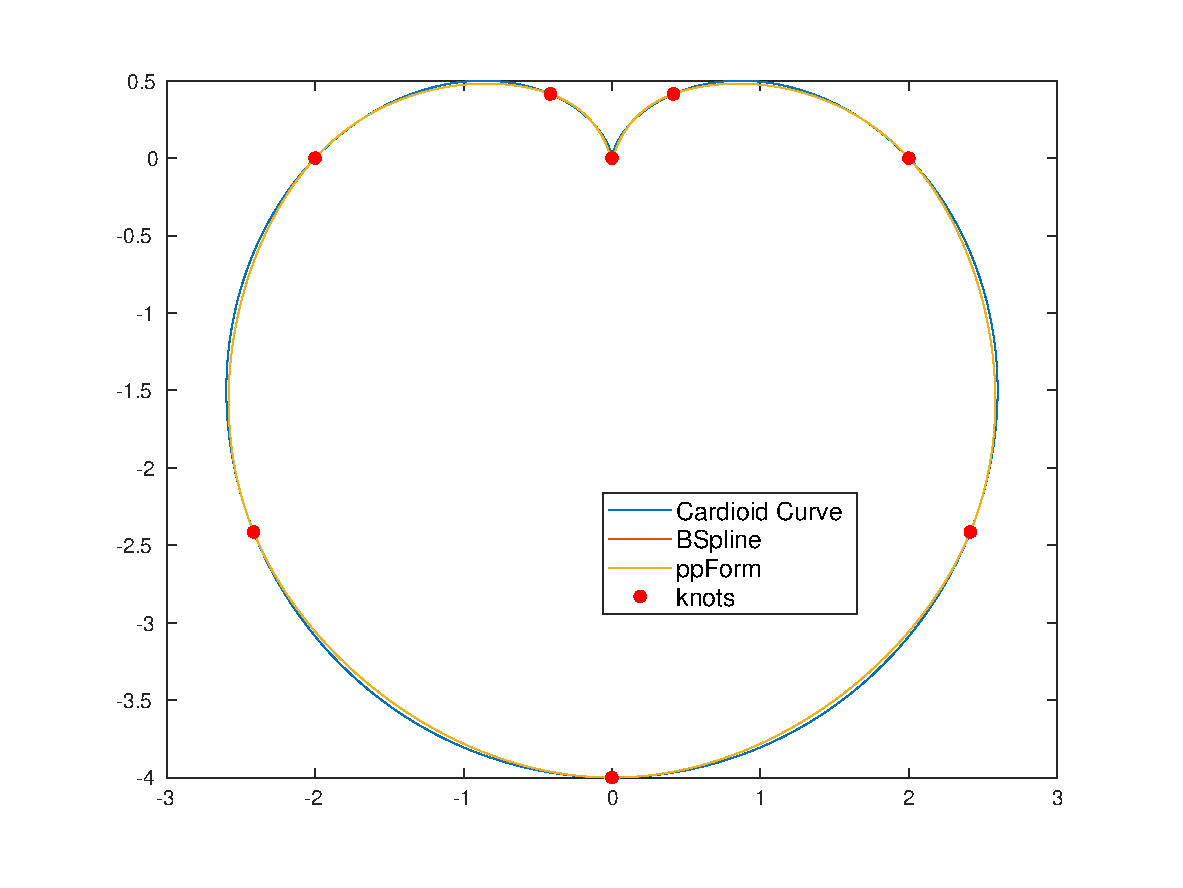
\includegraphics[width=0.9\linewidth]{figure/curve_cardioid_periodic.eps}
        \caption{\textit{periodic}}
        \label{fig:side:c}
    \end{minipage}%
\end{figure}

The bondary \textit{natural} performed worse than others. The local behavior at the end sees figure 13-16.

\begin{figure}[htbp]
    \centering
    \begin{minipage}[t]{0.24\linewidth}
        \centering
        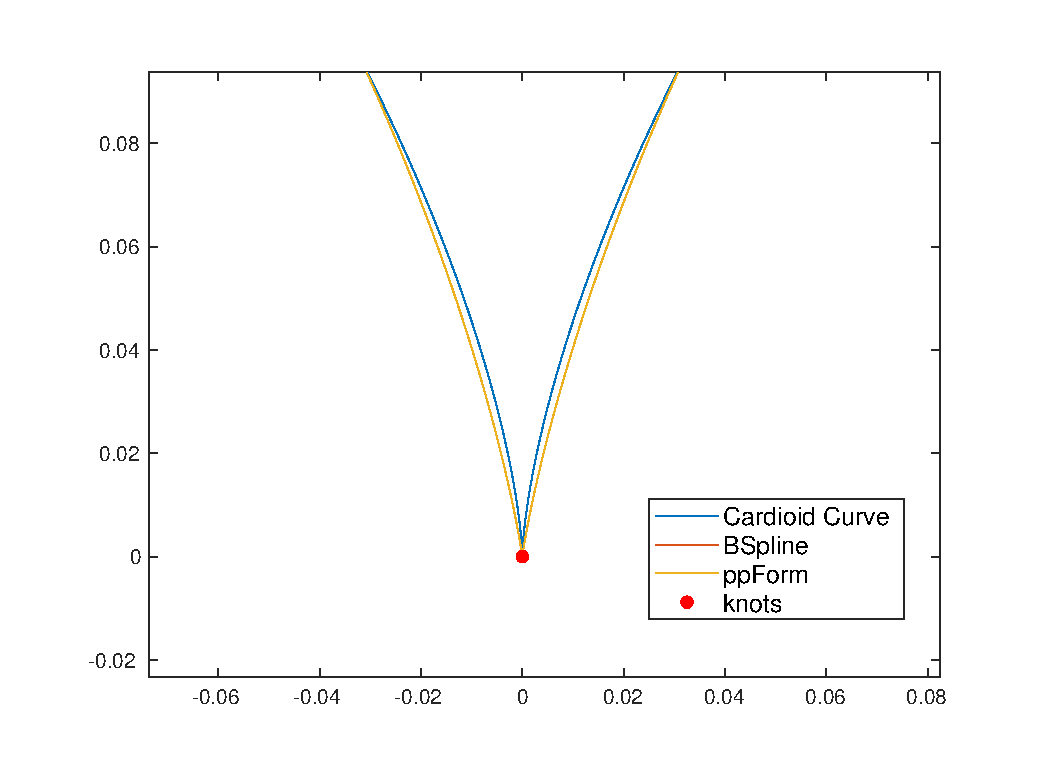
\includegraphics[width=0.9\linewidth]{figure/curve_cardioid_complete_local.eps}
        \caption{\textit{complete}}
        \label{fig:side:a}
    \end{minipage}%
    \begin{minipage}[t]{0.24\linewidth}
        \centering
        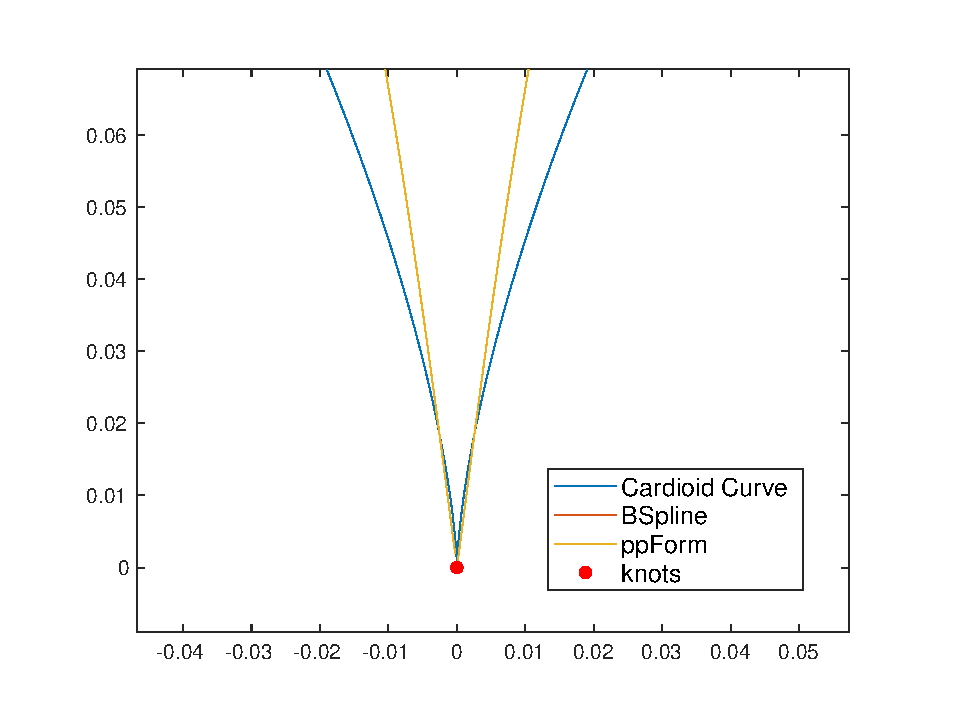
\includegraphics[width=0.9\linewidth]{figure/curve_cardioid_natural_local.eps}
        \caption{\textit{natural}}
        \label{fig:side:b}
    \end{minipage}
    \begin{minipage}[t]{0.24\linewidth}
        \centering
        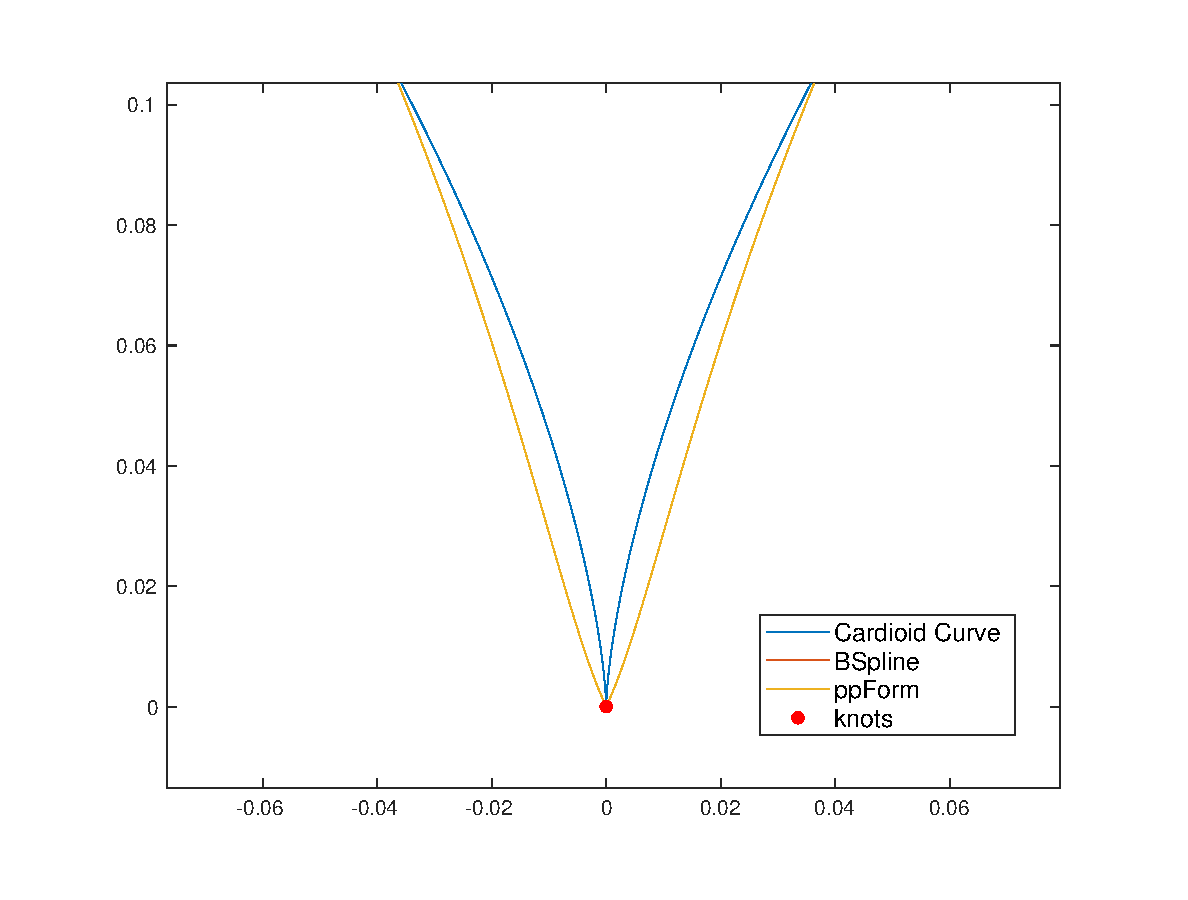
\includegraphics[width=0.9\linewidth]{figure/curve_cardioid_second-derivatives-at-end_local.eps}
        \caption{\textit{second-derivatives-at-end}}
        \label{fig:side:c}
    \end{minipage}%
    \begin{minipage}[t]{0.24\linewidth}
        \centering
        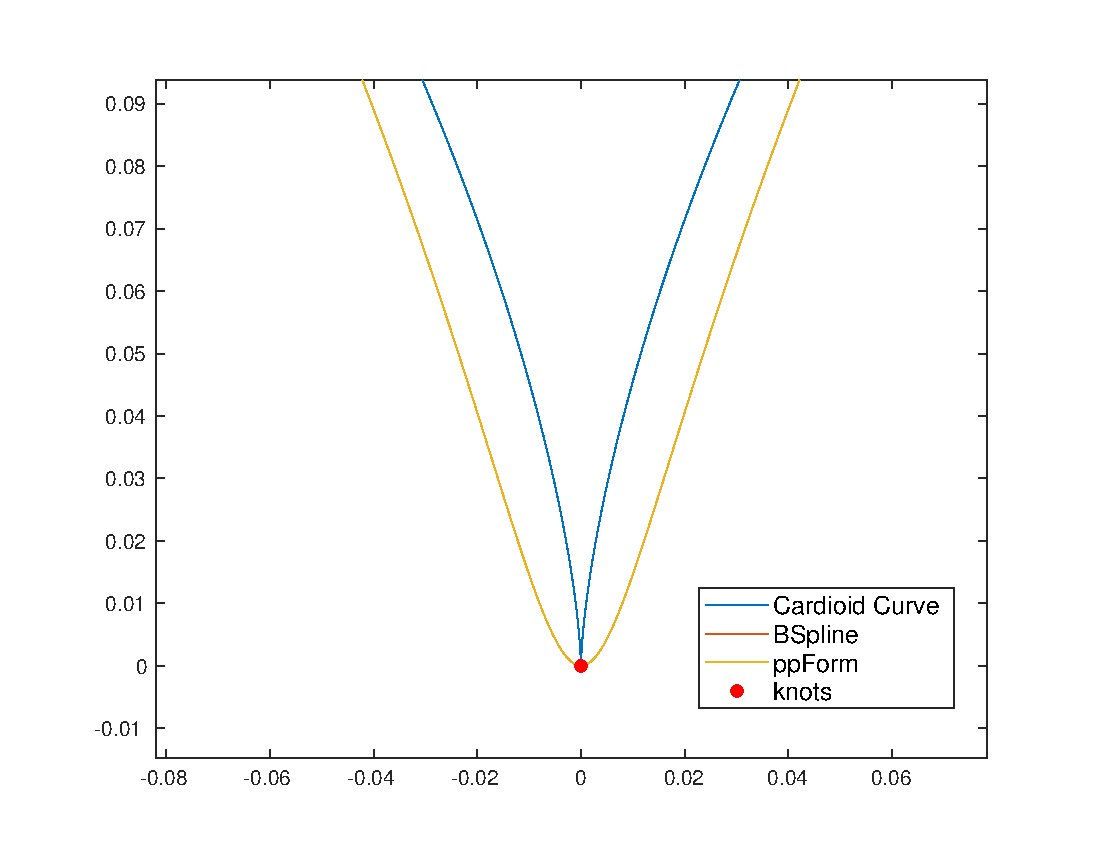
\includegraphics[width=0.9\linewidth]{figure/curve_cardioid_periodic_local.eps}
        \caption{\textit{periodic}}
        \label{fig:side:c}
    \end{minipage}%
\end{figure}

The end of periodic curve is smooth while others are sharp.

\section{Programming Assignments}

\end{document}
